\documentclass[draftthesis,fullpage]{uiucthesis2009}
%\documentclass[fancy,fullpage]{uiucthesis2009}
\usepackage[usenames,dvipsnames]{color}

\usepackage{graphicx}


\newcommand{\done}[1]{
\item{\textcolor{Green}{#1}}
}

\newcommand{\notdone}[1]{
\item{\textcolor{BrickRed}{#1}}
}

\newcommand{\itemheader}[1]{
\item{\textbf{#1}}
}

\newcommand{\statement}[1]{
\item{#1}
}

\newcommand{\tempfigure}[1]{

\begin{figure}[h]
\caption{#1}
\end{figure}
}

\begin{document}

\msthesis
\department{Materials Science and Engineering}
\advisor{Jennifer Lewis}
\title{Fabrication, self-assembly and dynamics of anisotropic colloids}
\author{Adam DeConinck}
\schools{B.S. Physics, Michigan Technological University, 2007}
\committee{Professor Jennifer A. Lewis}

\maketitle

\frontmatter

\begin{abstract}
This work details the development of techniques to fabricate and study structured colloidal particles...
\end{abstract}

\begin{dedication}
To Leigh.
\end{dedication}

\chapter*{Acknowledgements}

Any scientific project which is not completely trivial is the work
of many different people, and this project is no exception.  
First of all I would like to thank my advisor, Professor Jennifer
Lewis: without her ideas and support this project would simply
not exist, and her guidance has been crucial throughout my work.
Professor Jacinta Conrad and Dr.
Robert Shepherd were immensely important to this work, 
providing assistance and support throughout 
most of my graduate career.  They taught me everything I know 
about working with colloidal materials and microfluidics, and were
kind enough to answer many questions which I often could not even
properly articulate.  I owe special thanks to my undergraduate
assistants, Alissa Cote, Stephen Menke, Fatima Salazar and 
Kundan Chaudhary: they all spent a lot of time on that microscope
with me, and I can't imagine how I could have done without them.
I would also like to thank the rest of the Lewis Group for 
many things, great and small and too numerous to mention, all of
which made my life much easier; in particular Chris Hansen,
John Vericella, David Lorang, Elizabeth Glogowski and Willie Wu.
And Steve Kranz, who is taking over much of my work in the Lewis
group, I thank and wish good luck.

As much as graduate school seems to be the entirety of one's life
while it's going on, the rest of the world does in fact exist! 
With this in mind I would also like to extend thanks to those
who transformed these years of my life into more than one long 
slog in the lab. Mom, Dad and Brian were my rocks, and more important
than I can express without adding a second volume to this book.  
Dr. Huaibin Zhang was kind enough to give me fascinating things to
work on when I wasn't busy with this thesis; and Max, Phil and Steve
gave me games to play when I was done with that, too.  
The Lewis group as a whole have been more than just my colleagues,
and I thank them all for much fun and merriment. Dorian, Moki, 
and Tink have been the truest friends I had when I needed them most, 
and deserve all the thanks and praise I can give them.  And most of 
all I thank Leigh, without whom I would still be lost and alone in the
woods.  This is for you.

I know I've left people out, and to them I give my sincerest apologies.
I could not list everyone without destroying the illusion that this 
work is, in fact, about colloids.
The past few years have been hard and crazy and amazing, and I wouldn't trade them for
anything.  Thank you all.


\tableofcontents
\listoffigures

\mainmatter

\chapter{Introduction}

\begin{figure}
\begin{center}
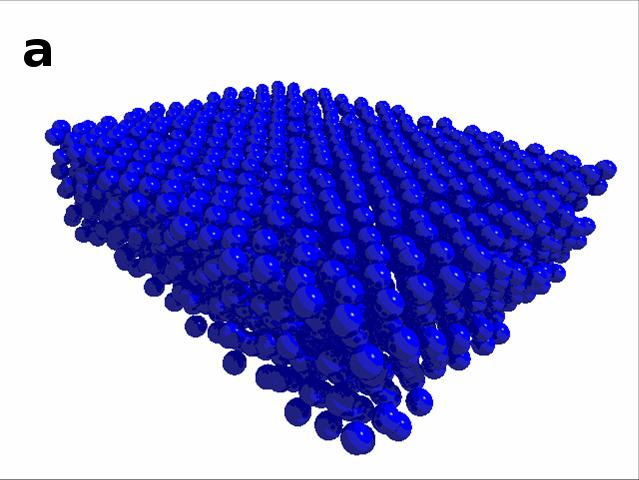
\includegraphics[height=1.5in]{figures/literature-review/sphere-crystal.png}
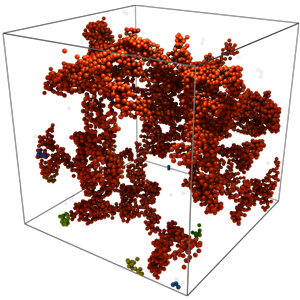
\includegraphics[height=1.5in]{figures/literature-review/sphere-gel.png}
\end{center}
\caption{Spherical colloids with purely repulsive interactions may assemble into (a) ordered 
crystal structures with fcc geometry or (b) open ``gel'' structures.}

\label{fig:isotropic-structs}

\end{figure}

As a class of materials, self-assembled colloidal structures are of interest in applications as widely varied
as photonic crystals~\cite{vos-photonic, yang-photonic} and three-dimensional templates for tissue 
engineering scaffolds~\cite{zhang-tissue}. However, despite the wide interest in these materials, the range of possible 
structures made available by self-assembled spherical colloids is relatively narrow.  Due to the isotropic nature
of colloidal interactions, there are two assembled structures available.
When the interparticle interaction is purely 
repulsive, such as in a hard-core interaction,  a stable, ordered face-centered-cubic crystal
structure(Fig.~\ref{fig:isotropic-structs}(a)) with a volume fraction of 0.54 is formed.~\cite{ise-crystal, wong-crystal}
When the interparticle interaction is attractive, the particles may form an open, disordered ``gel'' 
structure (Fig~\ref{fig:isotropic-structs}(b)) 
with an essentially random arrangement and gap volumes which are potentially larger than the 
particle size~\cite{warren-gel}.

Many applications, such photonic crystals, would benefit from the availability of different
kinds of self-assembled structures.~\cite{glotzer-solomon}  One way to address this is to 
introduce colloidal particles which incorporate one or more forms of anisotropy, in which the 
particle is altered such that the interaction between two or more particles becomes non-uniform depending on 
their relative orientations.  These alterations may be based on the shape of the particles, the chemical makeup, or 
some combination of the two.

\begin{figure}[h]
\begin{center}
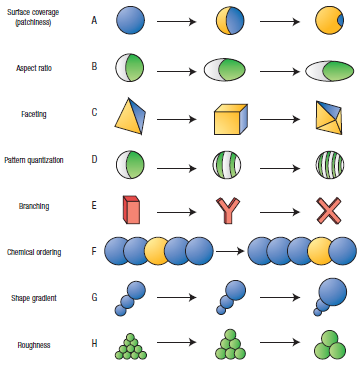
\includegraphics{figures/glotzer-anisotropy-dimensions.png}
\end{center}
\caption{Anisotropy dimensions proposed by Glotzer and Solomon~\cite{glotzer-solomon} to classify 
different forms of particle anisotropy.}
\label{fig:glotzer-dimensions}
\end{figure}


% Find many of the references in the following paragraph in Glotzer and Solomon's 2007 NatMat paper.
In a 2007 article in \textit{Nature Materials}~\cite{glotzer-solomon}, Glotzer and Solomon propose a system of anisotropy 
dimensions shown in Fig.~\ref{fig:glotzer-dimensions}. These include shape-based dimensions such as aspect 
ratio, faceting, branching, shape gradient 
and roughness (Fig.~\ref{fig:glotzer-dimensions}(B,C,E,G,H)) and dimensions based on the presence of
multiple chemistries such as surface coverage, pattern quantization and chemical ordering 
(Fig.~\ref{fig:glotzer-dimensions}(A,D,G)).  These dimensions do not necessarily 
represent an exhaustive list of the types
of anisotropy which are theoretically possible, but are a list of anisotropy types which have been observed in the
recent literature.  For example, rod-shaped or ellipsoidal particles of moderate aspect ratio have been fabricated 
by a wide variety of techniques including 
lithography~\cite{desimone-shear} and the stretching of colloidal spheres~\cite{rods-mohraz}; branched 
tetrapods have been fabricated of gold~\cite{gold-tetrapods},
and CdTe~\cite{cdte-tetrapods}; and chemically patterned particles have been produced
through microfluidic means~\cite{shepherd-janus}
as well as by conventional photolithography~\cite{desimone-janus}.  This list of dimensions may therefore
be seen as a useful framework for classification: by combining multiple dimensions, more complex types of particles may be 
developed (Fig.~\ref{fig:dimensions-combined}), or a complex particle may be classified in terms of which dimensions it includes.
New forms of anisotropy may be identified as those which cannot be decomposed into dimensions already identified.

\begin{figure}[h]
\begin{center}
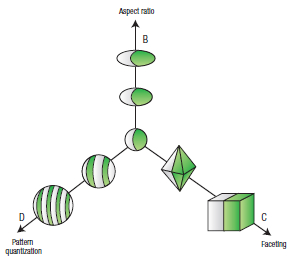
\includegraphics{figures/glotzer-combine-dimensions.png}
\end{center}
\caption{Multiple anisotropy dimensions may be combined to yield more complex types of particles.~\cite{glotzer-solomon}}
\label{fig:dimensions-combined}
\end{figure}

In this work, we develop techniques for
the fabrication of colliods with geometric and chemical anisotropy and begin to characterize the dynamical behavior
and self-assembly of these particles.

\section{Thesis Scope}

The aim of this work is to develop techniques for the fabrication and characterization of anisotropic colloids, and begin
to explore their dynamical and self-assembly behavior.  Fabrication is based on flow lithography
techniques for producing polymeric particles~\cite{dendukuri-cfl, dendukuri-sfl}, 
and characterization is primarily based on fluorescence and confocal 
microscopy~\cite{weitz-confocal} and particle 
tracking.~\cite{crocker-grier-spheres,rods-mohraz}
The systems used are based on a combination of a hydrophobic monomer (tri(methylol propane) triacrylate) and hydrophilic 
monomers (poly(ethylene glycol) diacrylate and 20-mol ethoxylated tri(methylol propane) triacrylate). 
Single-component particles are used to study the effects of
geometry on dynamical behavior in isolation, while multiple-component particles introduce 
the hydrophobic attraction for self-assembly.  The solvents used are 
varied to explore this interaction, and include
water, ethanol, dimethyl sulfoxide, isopropanol and toluene.

\section{Thesis Organization}

Chapter~\ref{ch:comp-tracking}
details algorithms and software developed in the course of this study to analyze microscopy images containing 
anisotropic colloids.  Chapter~\ref{ch:rods} investigates the fabrication, behavior and self-assembly of simple rod-shaped colloids
in both single-component and ``Janus'' forms, while Chapter~\ref{ch:exotic} 
investigates colloids with more exotic geometries. The main
conclusions are presented in Chapter~\ref{ch:conclusions}.  
Appendix~\ref{sec:matlab-implementation} details the Matlab implementation of the algorithms developed in
Chapter~\ref{ch:comp-tracking}.


\chapter{Literature Review}

\section{Introduction}

This literature review begins with an introduction to current work on the design and classification of 
anisotropic colloidal particles, and examples of real-world systems incorporating colloidal anisotropy.
This is followed by a discussion of current techniques for the fabrication of anisotropic colloids,
the theory of their self-assembly and experimental results.  Flow lithography is then reviewed in detail
to explore different forms of anisotropy which may be targeted by this technique.  Finally we review the current
state-of-the-art in the characterization of colloidal suspensions by particle tracking in microscopy image data, and
potential extensions of this technique for tracking anisotropic particles.

\section{Anisotropic and Patchy Colloids}

\subsection{Dimensions of Anisotropy}

\begin{figure}[h]
\begin{center}
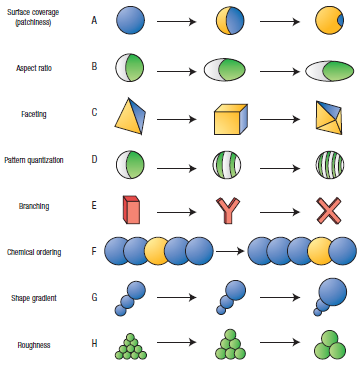
\includegraphics{figures/glotzer-anisotropy-dimensions.png}
\end{center}
\caption{Anisotropy dimensions proposed by Glotzer and Solomon~\ref{glotzer-solomon-assembly} to classify 
different forms of particle anisotropy.}
\label{fig:glotzer-dimensions}
\end{figure}

While the self-assembly of colloidal particles can produce structures with a variety of potential applications~\ref{??}, 
the range of structures which may be produced by conventional spherical colloids is limited.  One way to address this is to 
introduce colloidal particles which incorporate one or more forms of anisotropy, in which the 
particle is altered such that the interaction between two or more particles becomes non-uniform depending on 
their relative orientations.  These alterations may be based on the shape of the particles, the chemical makeup, or 
some combination of the two.

% Find many of the references in the following paragraph in Glotzer and Solomon's 2007 NatMat paper.
In a 2007 article in \textit{Nature Materials}~\ref{glotzer-solomon-assembly}, Glotzer and Solomon propose a system of anisotropy 
dimensions shown in Fig.~\ref{fig:glotzer-dimensions}. These include shape-based dimensions such as aspect 
ratio, faceting, branching, shape gradient 
and roughness (Fig.~\ref{fig:glotzer-dimensions}(B,C,E,G,H)) and dimensions based on the presence of
multiple chemistries such as surface coverage, pattern quantization and chemical ordering 
(Fig.~\ref{fig:glotzer-dimensions}(A,D,G)).  These dimensions do not necessarily 
represent an exhaustive list of the types
of anisotropy which are theoretically possible, but are an observational list of anisotropy types which have been observed in the
recent literature.  For example, rod-shaped or ellipsoidal particles of moderate aspect ratio have been fabricated 
by a wide variety of techniques including lithography~\ref{??} and particle distortion~\ref{solomon-confocal}; branched 
tetrapods have been fabricated of gold~\ref{??} and CdTe~\ref{??}; and chemically patterned particles have been produced
through microfluidic means~\ref{??} as well as by conventional photolithography~\ref{??}.  This list of dimensions may therefore
be seen as a useful framework for classification: by combining multiple dimensions, more complex types of particles may be 
developed (Fig.~\ref{fig:dimensions combined}), or a complex particle may be classified in terms of which dimensions it includes.
New forms of anisotropy may be identified as those which cannot be decomposed into dimensions already identified.

\begin{figure}[h]
\begin{center}
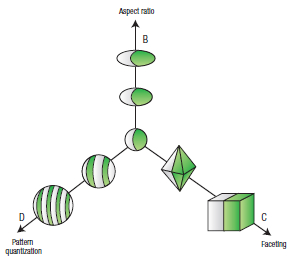
\includegraphics{figures/glotzer-combine-dimensions.png}
\end{center}
\caption{Multiple anisotropy dimensions may be combined to yield more complex types of particles.~\ref{glotzer-solomon-assembly}}
\label{fig:dimensions-combined}
\end{figure}

\begin{figure}[h]
\begin{center}
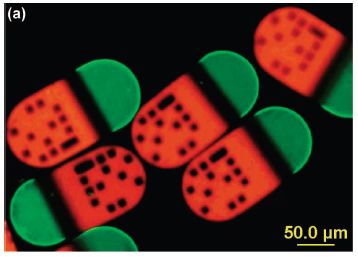
\includegraphics{figures/tan-dna-barcode.png}
\end{center}
\caption{``Barcoded'' PEG-DA particles which incorporating a DNA probe and fluorescent dyes~\ref{tan-barcode}.}
\label{fig:tan-particles}
\end{figure}

As an example of a particle which combines many types of anisotropy, 
consider the ``barcoded'' particles described in \textit{Tan et al.}~\ref{tan-barcode} for DNA analysis (Fig~\ref{fig:tan-particles}).
These particles have multiple aspect ratios (dimension B); faceting, due to the flat top and bottom surfaces (C); and pattern
quantization due to the three different chemistries included (D).  An additional form of anisotropy, the barcoding, may be seen
as a new dimension or as a more complex instance of pattern quantization.  While these particles are larger than typical colloidal
dimensions, they illustrate these principles vividly and it is reasonable to suspect they may be miniaturized.

\subsection{Theory of self-assembly}
\begin{figure}
\label{fig:glotzer-sim-assembly}
\end{figure}

\subsection{Fabrication of anisotropic colloids}

\begin{figure}
\caption{Janus spheres fabricated by emulsion technique~\ref{granick-janus}.}
\label{fig:granick-janus-spheres}
\end{figure}

\begin{figure}
\caption{PMMA rods are fabricated by (a) embedding PMMA spheres in PDMS, (b) stretching the PDMS while heated and allowing it 
it to cool, and (c) dissolving the PDMS to reveal ellipsoidal rods.}
\label{fig:solomon-rods}
\end{figure}

\begin{figure}
\label{fig:branched-particles}
\end{figure}

\begin{figure}
\label{fig:faceted-particles}
\end{figure}

\begin{figure}
\label{fig:PRINT}
\end{figure}

\begin{itemize}
\statement{Fabrication of Janus spheres: Granick, etc}
\statement{Fabrication of rods}
\statement{Fabrication of Janus rods}
\statement{Faceted particles (crystal growth etc)}
\statement{Flow lithography}
\statement{PRINT particles}
\end{itemize}


\begin{itemize}
\statement{Glotzer work on spherical patchy colloids}
\statement{Other self-assembly of spherical colloids}
\statement{Review self-assembly of non-spherical patchy colloids: focus on Janus rods}
\end{itemize}

\subsection{Experimental self-assembly}
\tempfigure{Small clusters of Janus spheres; wormlike chains; Granick}
\tempfigure{Multi-panel figure: other assembly}
\begin{itemize}
\statement{Hydrophobic/hydrophilic: Granick, clusters}
\statement{Charge-based assembly}
\statement{Magnetic assembly}
\statement{DNA-based assembly}
\end{itemize}

\section{Flow Lithography}

\begin{itemize}
\statement{Doyle: continuous-flow lithography}
\statement{Stop-flow lithography}
\statement{Multiple-stream particles}
\statement{Applications: biomolecules, etc}
\statement{Recent elaborations: lock-release, phase mask, etc}
\end{itemize}

\section{Particle Tracking}

\tempfigure{Particle tracking illustration}
\tempfigure{Solomon rod tracking}
\tempfigure{Illustrate morphological processing}
\begin{itemize}
\statement{Crocker and Grier: IDL particle tracking}
\statement{Solomon: rod particle tracking}
\statement{Other relevant tracking?}
\statement{Basic review of morphological image processing}
\end{itemize}


\chapter{Computerized Tracking of Anisotropic Colloids}
\section{Introduction}

Confocal laser scanning microscopy (CLSM) is a powerful technique for the study of three-dimensional
structure in fluorescent materials. When applied to fluorescent colloids, CLSM enables the observation
and identification of individual particles, determining their positions in three-dimensional space.
These particle locations alone can be used to derive a great deal
of information about the material, such as the distribution of number of nearest neighbors and
the pair distribution function (PDF). Repeated observations at regular intervals allow for dynamical
measurements of parameters such as the diffusion constant, and may be used to study the microstructual
differences between different parts of the colloidal phase diagram. CLSM has the additional advantage
that since it produces real-space position data, it has substantial advantages over scattering techniques
in coping with samples with highly asymmetric structures.~\ref{?}

However, 
the production of 3D structural information requires more than just a powerful imaging technique: it also
requires powerful computational analysis to translate image data into a list of particles and positions, and
to determine the relevant physical data from this list.  In addition, the behavior of non-spherical colloids
is governed not only by the relative positions of the particles but also their orientations. Developing an
understanding of anisotropic colloids
therefore calls for the development of image processing techniques for the extraction and analysis of
structural data from microscopy images.

\section{Literature review}

\subsection{Particle tracking with spherical colloids}

The current state of the art in 

\subsection{Solomon rod tracking}

\tempfigure{Illustration of Solomon technique}
\tempfigure{SFL particles as 2D extruded objects; flat fluorescence}
\begin{itemize}
\statement{Desirable to locate anisotropic particles in microscopy images to study dynamics and assembly.}
\statement{Previous work in this area: Crocker and Grier, Solomon}
\statement{Can't use Solomon method: fluorescence is too flat for SFL particles. 2D-extruded objects. (Figure to illustrate.)}
\statement{Must develop new algorithms which can work on these particles.}
\end{itemize}

\section{Rod-tracking algorithm}

Our algorithm for locating and tracking SFL rods draws heavily from the algorithm published by 
Mohraz and Solomon for tracking PMMA rods.~\ref{moraz-solomon-rods}.  Briefly, this algorithm 
took advantage of the gradient in fluorescent intensity throughout the volume of the 
rods they studied, which were fabricated by stretching spherical PMMA particles along a single axis.
Because these rods had a circular cross-section, scanning the confocal laser through a point nearer
to the rod axis would pass through a greater volume of fluorescent material, producing a higher intensity.
By applying a local line maximum criterion to the points inside the particle volume, they were able to 
build a ``backbone'' of points near the axis, allowing them to reliably calculate orientation.

While this algorithm performs very well for a restricted class of rods, it fails in cases where the particle
cross-section is not circular, and points near the particle backbone are not guaranteed to produce higher 
intensities than their immediate neighbors.  This is the case for our ``rods'' produced by stop-flow
lithography (SFL), in which the sides of the rods are relatively flat due to the fabrication
geometry. These particles have correspondingly flat fluorescence profiles, and require a more complex analysis
to calculate a ``backbone''.

We have developed an algorithm for processing 2D and 3D CLSM data of fluorescent SFL rods to
produce position and orientaion data.  Starting from raw CLSM images, this algorithm can be divided
into several phases, including (i) image cleanup; (ii) segmentation; (iii) skeletonization;
(iv) position calculation; and
(v) particle tracking over the time series.  

A note on terminology: the algorithm described below is identical for both 2D and 3D images, as all
operations are defined for both cases and used identically. However, where the individual elements of
2D images are referred to as pixels, the elements of 3D images are generally referred to as voxels.
For simplicity, all such elements are referred to as pixels in the explanation below.

\subsection{Image cleanup}

Two different image cleanup methods were considered, and used depending on their effectiveness with
sample data.

The first method, a real-space bandpass filter, is derived from the filter published in the 
Matlab implementation of spherical particle tracking~\ref{crocker-weeks} by Blair and
Dufrense. This filter performs a band-pass by convolving the image with two kernels: 
a Gaussian kernel and a boxcar kernel.  The Gaussian convolution performs the low-pass
operation, while subtracting the result of the boxcar convolution from the Gaussian result
performs the high-pass operation. This filter takes two parameters, the characteristic scale
of image noise (generally equal to one pixel) and the typical particle size.  This works well,
but has issues in images with multi-pixel noise.

While the band-pass performed well on most images, some experiments produced data with noise or
extraneous features which did
not easily yield to the bandpass operation. This can be attributed to the fact that SFL fabrication produces
solutions which have some amount of fluorescent monomer present in the liquid as well as the particles, which
could not always be removed effectively.  A second method was devised using morpholohical
operations to better neutralize non-particle features.

This method may be divided into four steps. First the image is thresholded to produce a binary image, where the 
background is black and the fluorescent features are white. The threshold is selected such that pixels which 
are part of the particle volume are never assigned to the background; Otsu's criterion was found to be reliable
for this.~\ref{?}  Second, a binary opening is applied with an isotropic structuring element to
suppress small features. The size of the structuring element is selected manually by the user, but a 
reliable choice was found to be a diameter roughly equal to half the width of the typical rod. 

At this point a binary image has been produced which suppresses most non-particle features, but morphological
image operations are not guaranteed to preserve shape and orientation of image features.  To retain the noise suppresion
but regain the original shape, we perform one additional morphological dilation using the same structuring element to
guarantee that the foreground regions fully overlap with the rods, then perform a binary AND between the result and the
original image. This is effectively equivalent to using the result of our morphological operations as a mask on
the original, suppressing
all pixels which are marked as background.

\subsection{Segmentation}

The next step of the algorithm is image segmentation, in which individual particles are identified and each pixel
in the image is 

\tempfigure{Image processing flowchart}
\tempfigure{Example image: cleanup, segmentation, skeleton, track}
\tempfigure{Schematic comparison of 2D/3D}
\tempfigure{Schematic explanation of ``template'' technique for tracking arbitrary shapes}
\tempfigure{Example images for ``template'' tracking}
\begin{itemize}
\done{Tracking algorithm for rods}
\begin{itemize}
\done{Image cleanup using erosion, opening}
\done{Particle segmentation using watershed transform}
\done{Particle skeleton (backbone) using distance transform plus rank-order filter}
\done{Calculation of center-of-mass, oritentation according to Solomon}
\done{Time-series tracking according to Blair and Dufrense}

\done{Difference between 2D and 3D version of algorithm}

\end{itemize}

\notdone{Tracking algorithm for arbitrary shapes}

\begin{itemize}
\done{Initial steps same as for rods: cleanup, segmentation}
\done{``Skeletonization'' as above, but producing a more complex skeleton than for rods}
\done{Calculate center-of-mass as with rods}
\done{Choose a sample skeleton as the ``canonical'' particle skeleton}
\done{Isolate particles into individual windows}
\done{To measure orientation: rotate canonical skeleton image in small increments. For each one, AND together the 
rotated skeleton and the sample skeleton.  Maximize pixel sum of ANDed image.}
\done{Faster in 2D than in 3D}
\notdone{Implementation not finished!}
\end{itemize}

\end{itemize}

\section{Implementation}

\tempfigure{Example particle tracks}
\begin{itemize}
\done{Rod tracking implemented in 2D in Matlab.}
\statement{Go over the details of the matlab implementation}
\notdone{Rod tracking implemented in 3D in Matlab, but with major bugs.}
\notdone{Arbitrary tracker not yet fully implemented, using Matlab.}
\end{itemize}

\section{Assessment}

\tempfigure{Cartoons to show possible errors}
\begin{itemize}
\done{Identify issues caused by morphological image processing for these algorithms.}
\notdone{Estimate errors in particle segmentation}
\notdone{Estimate error of rod COM and orientation calculations.}
\notdone{Estimate error of skeleton-based orientation calculations.}
\end{itemize}


\chapter{Assembly and Dynamics of Rod-Shaped Colloids}
\section{Introduction}



\tempfigure{Colloidal rod examples}
\begin{itemize}
\statement{Natural rod systems}
\statement{Systems studied by Solomon}
\statement{Janus colloids: Granick}
\statement{Interest in Janus rods}
\end{itemize}

\section{Literature Review}

\section{Experimental Procedure}
\subsection{Stop-Flow Lithography}

\tempfigure{Photo of SFL setup; SFL flowchart; example experiment}
\begin{itemize}
\done{Microscope setup}
\done{Pressure system--Rob}
\done{LabView controller for SFL}
\done{Design of microfluidic devices for up to 3-stream SFL}
\done{Fabrication of microfluidic devices}
\end{itemize}

\tempfigure{Examples of SFL masks used in rod experiments}
\subsection{Mask Design}
\begin{itemize}
\done{Demagnification using 60X objective}
\done{Design parameters}
\done{Rod aspect ratios used}
\end{itemize}

\subsection{Particle Collection}
\begin{itemize}
\done{Considerations for collection}
\done{Solvents used}
\done{Pipettes}
\done{Fluorosilane coatings}
\end{itemize}

\subsection{Diffusion Measurements}
\begin{itemize}
\done{Confocal microscopy setup}
\done{Space and time resolution requirements}
\done{Fluorescence requirements}
\end{itemize}

\section{Results and Discussion}

\tempfigure{Resolution test mask; image of resulting particles}
\subsection{Resolution}
\begin{itemize}
\done{Limiting factors for SFL resolution: mask design, optics, flow effects}
\notdone{Resolution limits constrained by 60X lens--need to redo this (~1 hour work)}
\done{Resolution limits for Janus rods--interface effects}
\end{itemize}

\tempfigure{Image of rod tracking}
\tempfigure{Plots of translational and rotational diffusion data}
\subsection{Translational and Rotational Diffusion}
\begin{itemize}
\done{Particle collection--PEGDA vs TMPTA}
\done{Compare particle/solvent/surface effects}
\notdone{2D diffusion size series: TMPTA in toluene (additional experiments may be required)}
\notdone{Analyze diffusion data for rods (partially done).}
\end{itemize}

\tempfigure{Show fabricated Janus rods of various sizes.}
\tempfigure{Assembly of rods in various solvents}

\begin{figure}
\begin{center}
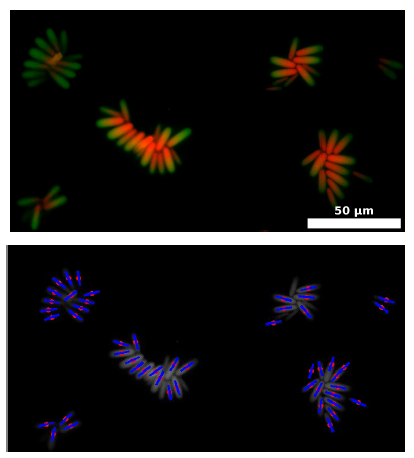
\includegraphics{figures/assembled-janus-tracked.png}
\end{center}
\caption{(a) Janus rods which have self-assembled into ordered 
clusters are identified and separated, and (b) their 
positions and orientations are labeled.}
\label{fig:assembled-janus-tracking}
\end{figure}

\subsection{Self-Assembly of Janus Rods}
\begin{itemize}
\done{Fabrication of Janus rods: various sizes (figure)}
\done{Comparison of self-assembly in various solvents (figure)}
\done{Small clusters vs large structures}
\done{Alignment of assembled rods}
\done{Image segmentation for analyzing structures}
\notdone{Some more good-looking images may be required}
\end{itemize}


\chapter{Assembly and Dynamics of Exotic Colloids}

\section{Introduction}

\tempfigure{Glotzer anisotropy dimensions targeted by complex SFL}
\begin{itemize}
\statement{Motivation for working on more complex shapes}
\statement{Reference Glotzer anisotropy dimenions}
\statement{Bring back three-stream SFL concept from lit review}
\end{itemize}

\section{Experimental Procedure}
\subsection{Device Design}

\tempfigure{Schematic for 3-stream channel, and constriction channel}
\begin{itemize}
\done{Design for three-stream SFL microfluidic device: explain considerations}
\done{Channel-constriction design}
\end{itemize}

\subsection{SFL with Multiple Co-Flowing Streams}

\begin{itemize}
\itemheader{Alterations necessary to SFL protocol with three streams}
\begin{itemize}
\done{Timing considerations}
\done{Pressure considerations}
\end{itemize}
\end{itemize}

%\subsection{Mask Design}
%\subsection{Particle Collection}

\section{Results and Discussion}

\subsection{SFL limitations}

\tempfigure{Show stable parallel interface vs droplet forming}

\begin{itemize}
\done{Multiple streams result in SFL slowdown}
\notdone{Theoretical constraints on how closely interfaces can be spaced}
\done{Empirical comparsion on interface spacing}
\end{itemize}

\subsection{Particles produced}


\tempfigure{Figure showing 2, 3, 4 patch particles}
\tempfigure{Figure showing boomerangs, and self-assembly concept}
\begin{itemize}
\done{Family of particles produced}
\done{Branched (multi-patch) particles (figures)}
\done{Boomerang fabrication and concept}
\end{itemize}

\tempfigure{Diffusion results for complex particles}
\subsection{Diffusion Measurements}
\begin{itemize}
\notdone{Confocal measurements of 2D diffusion for various shapes--not systematically done}
\notdone{Diffusion results}
\end{itemize}

\subsection{Self-Assembly}

\tempfigure{Show two-patch self-assembly}
\tempfigure{Show samples with little assembly; schematic of surface effects}
\begin{itemize}
\done{Some self-assembly observed for two-patch rods}
\done{Little self-assembly observed for larger, less mobile particles}
\done{Surface effects may affect observed assembly}
\end{itemize}

\chapter{Conclusions}

In this work we studied the fabrication, self-assembly and dynamical behavior
of shape- and chemically-anisotropic colloidal particles.  The fabrication 
of colloidal rods of various sizes and aspect ratios was demonstrated via
stop-flow lithography for rods with
hydrophilic, hydrophobic and Janus functionalities.  Image processing algorithms
were developed for identifying, locating and measuring the orientation of 
colloidal rods in microscopy images, and software was implemented to carry out
this analysis and characterize structural and dynamical properties.
Single-component particle 
dynamics were observed via time-series confocal microscopy using particles of 
various aspect ratios to study the effects of particle geometry on diffusion.
The self-assembly of Janus rods was studied using
3D confocal microscopy for particles of various aspect ratios,
in a number of different solvent conditions, to determine the effects of size 
and attraction strength on the resulting structure.  The fabrication of more complex
multiple-patch particles with several different geometries was also demonstrated via SFL.

\section{Future work}

Significant challenges were identified in the areas of particle collection and processing as 
detailed in Section~\ref{sec:rod-collection} which may have significantly affected the 
results of dynamics and self-assembly experiments.  It might be possible to solve these
processing issues using some non-stick coating instead of the fluorosilane coating 
which was used.  Another avenue to explore includes the use of a microfluidic concentration
and cleaning solution to exchange the monomer solution for another solvent, 
which may be integrated with the fabrication system.  

Once these issues have been solved, a number of interesting studies on the dynamics and
structure of suspensions of microfabricated colloids are possible.  This includes studying 
self-assembly and dynamics of colloidal suspensions at high concentrations, as well as 
the behavior of biphasic suspensions containing a mix of particles with different geometries and
functionalities.~\cite{?}

It should also be possible to develop image processing algorithms to track particles with more
complex geometries.  The algorithm developed in Chapter~\ref{ch:comp-tracking} is independent 
of particle geometry throughout the image cleanup, segmentaton and skeletonization steps.
The development of algorithms which could translate the skeletons of other particle 
geometries into position and orientation information would greatly expand the 
capabilities of particle tracking.


\appendix

\chapter{Microfluidic Devices for Studying Self-Assembly}
\section{Introduction}

\begin{itemize}
\statement{SFL is low-scale technique for fabricating very small particles}
\statement{Most interesting physics occurs at higher concentrations}
\statement{SFL yields are low once particles are transferred out of device}
\statement{Single microfluidic system to fabricate and study particles is desirable}
\end{itemize}

\section{Experimental Procedure}
\subsection{Device Design and Fabrication}

\tempfigure{Overall design}
\tempfigure{Post filters; Channel-height filters}
\begin{itemize}
\done{Design capable of multi-stream fabrication}
\done{Design capable of concentrating particles in a small container}
\done{Multi-layer SU-8 master fabrication}
\done{Initial filter design: posts}
\done{Final filter design: channel height}
\done{Concentrator geometries}
\done{System to exchange solvents and clean particles}
\end{itemize}

\subsection{Proposed Protocol}

\tempfigure{Cartoon of proposed protocol}
\begin{itemize}
\done{Fabricate particles in channel}
\done{Particles collect in concentration chamber}
\done{When finished, cure fab channel shut}
\done{Rinse particles}
\done{Agitate to break up structure}
\done{Image}
\end{itemize}


\section{Results and Discussion}

\subsection{Concentrator results}

\tempfigure{Janus particles in concentrator}
\tempfigure{Failed devices}
\begin{itemize}
\done{Particle fabrication: slowed by pressure}
\done{Particle concentration by filters}
\done{Solvent exchange: challenges due to pressure buildup}
\done{Aggregates refuse to break up: suggested explanations}
\done{Device failures}
\end{itemize}

\section{Future directions}

\begin{itemize}
\statement{Suggestions on device design}
\statement{Suggestions for other uses of these devices}

\end{itemize}


\chapter{Grayscale Stop-Flow Lithography}
\section{Introduction}

\begin{itemize}
\statement{SFL particle height set by channels; low versatility}
\statement{Allow height variation within channel?}
\statement{Give examples of grayscale lithography}
\end{itemize}

\section{Experimental Procedure}
\subsection{Design of Grayscale Filters}

\tempfigure{Plot transmission vs filter thickness}
\begin{itemize}
\done{Construct mixed-PDMS filters}
\end{itemize}

\subsection{Grayscale Stop-Flow Lithography}

\tempfigure{Cartoon of grayscale SFL fabrication}
\begin{itemize}
\done{Placement in SFL beam path}
\done{Experimental optimization}
\end{itemize}

\section{Results and Discussion}

\subsection{Resulting particles}
\begin{itemize}
\done{Achieved height variation}
\done{Particle swelling issues observed}
\end{itemize}

\section{Future work}
\begin{itemize}
\notdone{True grayscale masks}
\end{itemize}

\end{document}